% ============================================================
%  Diplomski rad — Alan Bubalo
%  Obrasci tolerancije na greške u distribuiranim sustavima:
%  studija slučaja Fiskalizacije 2.0
%
%  Build:  latexmk -pdf main.tex
%  Clean:  latexmk -c
% ============================================================
\documentclass[12pt,a4paper,oneside]{book}

% ============================================================
%  Preamble — paketi i postavke
% ============================================================

% ---- Kodiranje i jezik -------------------------------------
% Kodiranje T1 drži dijakritike kao jedan znak. U OT1 su složeni, pa đ ispada
% iz tekstualnog sloja PDF-a i pretraživanje ne nalazi riječi koje ga imaju.
\usepackage[T1]{fontenc}          % UTF-8 je zadan od LaTeX 2018, inputenc nije potreban
\usepackage{lmodern}
% Engleski je glavni jezik dokumenta, a hrvatski uključuje
% \selectlanguage{croatian} prije sadržaja u main.tex i vrijedi do kraja rada.
\usepackage[croatian,english]{babel}
\usepackage{csquotes}             % biblatex ga traži uz babel
% Babel prevodi \appendix kao „Dodatak"; u hrvatskim radovima je uvriježeno „Prilog".
\addto\captionscroatian{\renewcommand{\appendixname}{Prilog}}

% ---- Raspored stranice -------------------------------------
\usepackage{geometry}
\geometry{
  a4paper,
  left=1.25in,
  right=1.25in,
  top=1in,
}
\usepackage[hang,flushmargin]{footmisc}
\usepackage{microtype}

% Numeriraju se dvije razine naslova (4.1), niže ne. Poglavlje je \section,
% odjeljak \subsection. Pododjeljci idu kao \subsubsection* i \paragraph,
% bez broja i bez stavke u sadržaju.
\setcounter{secnumdepth}{2}
\setcounter{tocdepth}{2}

% ---- Grafika i tablice -------------------------------------
\usepackage{graphicx}
\graphicspath{{slike/}}
\usepackage{float}
% Širine stupaca u tablicama pisane su u dijelovima \textwidth, a ne u
% centimetrima, pa prate marginu i ne prelijevaju se kad se ona promijeni.
\usepackage{booktabs}
\usepackage{multirow}
\usepackage{array}
\usepackage{longtable}
\usepackage{caption}
\usepackage{subcaption}
\usepackage{xcolor}
\usepackage{enumitem}
% Za listinge koji se ne smiju odvojiti od svojeg opisa.
\usepackage{needspace}

% ---- Dijagrami (TikZ) --------------------------------------
\usepackage{tikz}
\usetikzlibrary{shapes.geometric, arrows.meta, positioning, fit, calc}

% ---- Matematika --------------------------------------------
\usepackage{amsmath}
\usepackage{amssymb}

% ---- Listanje koda (PHP / Laravel) -------------------------
\usepackage{listings}
\definecolor{codebg}{rgb}{0.97,0.97,0.97}
\definecolor{codekw}{rgb}{0.12,0.29,0.55}
\definecolor{codecomment}{rgb}{0.40,0.55,0.40}
\definecolor{codestring}{rgb}{0.60,0.20,0.20}
\lstdefinestyle{kod}{
  backgroundcolor=\color{codebg},
  basicstyle=\ttfamily\footnotesize,
  keywordstyle=\color{codekw}\bfseries,
  commentstyle=\color{codecomment}\itshape,
  stringstyle=\color{codestring},
  numbers=left,
  numberstyle=\tiny\color{gray},
  numbersep=8pt,
  breaklines=true,
    showstringspaces=false,
  % Fiksni stupci ubacuju razmake oko znakova koje listings vidi kao zasebne
  % tokene, pa se `--without-intent-record` ispisivao kao `-- without - intent`.
  % Fleksibilni stupci uz keepspaces to uklanjaju, a monospace font i dalje
  % drži poravnanje ASCII tablica u dokaznim ispisima.
  columns=fullflexible,
  keepspaces=true,
  frame=single,
  rulecolor=\color{gray!40},
  tabsize=2,
  captionpos=b,
  extendedchars=true,
  literate=%
    {č}{{\v c}}1 {ć}{{\'c}}1 {ž}{{\v z}}1 {š}{{\v s}}1 {đ}{{\dj}}1
    {Č}{{\v C}}1 {Ć}{{\'C}}1 {Ž}{{\v Z}}1 {Š}{{\v S}}1 {Đ}{{\DJ}}1
}
\lstset{style=kod}
\lstdefinelanguage{PHP}{
  morekeywords={abstract,and,array,class,const,echo,else,elseif,extends,
    final,for,foreach,function,if,implements,interface,namespace,new,
    private,protected,public,return,static,throw,try,catch,finally,use,
    while,yield,match,fn,enum,readonly,null,true,false},
  sensitive=true,
  morecomment=[l]{//},
  morecomment=[l]{\#},
  morecomment=[s]{/*}{*/},
  morestring=[b]",
  morestring=[b]'
}

% ---- Bibliografija -----------------------------------------
\usepackage[backend=biber,style=ieee,sorting=none]{biblatex}

% Stil ieee ne poznaje tipove @legislation i @standard, pa je bez ovih dviju
% naredbi ispisivao „No driver for..." i posezao za zamjenskim oblikovanjem.
% Aliasi taj izbor čine izričitim: propisi i norme oblikuju se kao @misc, koji
% ispisuje polje howpublished (npr. „Narodne novine, br. 89/2025").
\DeclareBibliographyAlias{legislation}{misc}
\DeclareBibliographyAlias{standard}{misc}

\addbibresource{references.bib}

% Bilješka koja se lomi između stranica teško se čita, a rad ima nekoliko
% dugih doslovnih citata u bilješkama. Visoka kazna TeX-u govori da radije
% pomakne odlomak nego da bilješku prelomi.
\interfootnotelinepenalty=10000

% ---- Poveznice (učitati pri kraju) -------------------------
\usepackage[hidelinks]{hyperref}
\usepackage{cleveref}
% Poglavlje je \section, pa nazivi idu jednu razinu niže od uobičajenih.
\crefname{section}{poglavlje}{poglavlja}
\Crefname{section}{Poglavlje}{Poglavlja}
\crefname{subsection}{odjeljak}{odjeljci}
\Crefname{subsection}{Odjeljak}{Odjeljci}
\crefname{figure}{slika}{slike}
\Crefname{figure}{Slika}{Slike}
\crefname{table}{tablica}{tablice}
\Crefname{table}{Tablica}{Tablice}

% ---- Pomoćne naredbe ---------------------------------------
% Oznaka za nedovršeni dio teksta. Ispisuje se crveno i ulazi u popis
% na kraju rada (\popistodo), da se nedovršeno ne izgubi iz vida.
\newcounter{todocnt}
\newcommand{\todo}[1]{%
  \stepcounter{todocnt}%
  \textcolor{red}{\textbf{[TODO \thetodocnt: #1]}}%
  \addcontentsline{tdo}{section}{\protect\numberline{\thetodocnt}#1}%
}
\makeatletter
\newcommand{\popistodo}{%
  \clearpage
  \section*{Popis nedovršenog}%
  \markboth{Popis nedovršenog}{}%
  \@starttoc{tdo}%
}
\makeatother

% Strani termin pri prvom spominjanju: \strani{prekidač}{circuit breaker}
\newcommand{\strani}[2]{#1 (\emph{#2})}

% Kratica pri prvoj uporabi: \kratica{puni naziv}{engleski izvornik}{KRATICA}
\newcommand{\kratica}[3]{#1 (engl.\ \emph{#2}, skraćeno #3)}
% Kratica bez ustaljenog hrvatskog naziva: \kraticaen{KRATICA}{engleski izvornik}
\newcommand{\kraticaen}[2]{#1 (engl.\ \emph{#2})}
% Domaća kratica, bez engleskog izvornika: \kraticahr{puni naziv}{KRATICA}
\newcommand{\kraticahr}[2]{#1 (skraćeno #2)}


% ---- Metapodaci rada ---------------------------------------
% Polja naslovnice slijede službeni obrazac UNIPU
% „Naslovna i prva stranica — diplomski rad", preuzet 2026-08-14.
%
% ⚠ SVE ŠTO JE U UGLATIM ZAGRADAMA POPUNJAVA SE PRIJE PREDAJE.
%   Ta polja ne ovise o sadržaju rada; popunjavaju se na kraju,
%   u jednom prolazu, i to je jedino mjesto na kojem se mijenjaju.
\newcommand{\radNaslov}{Obrasci tolerancije na greške u distribuiranim sustavima: studija slučaja Fiskalizacije 2.0}
\newcommand{\radNaslovEng}{Fault-Tolerance Patterns in Distributed Systems: A Case Study of Fiscalization 2.0}
\newcommand{\radAutor}{Alan Bubalo}
\newcommand{\radJmbag}{0303098591}
\newcommand{\radMentor}{[ime mentora]}
% FIPU nudi dva diplomska smjera: „Diplomski sveučilišni studij Informatika"
% i isti studij uz dodatak „nastavni smjer". Upisati onaj s upisnice.
\newcommand{\radSmjer}{[Diplomski sveučilišni studij Informatika?]}
\newcommand{\radPredmet}{[predmet pod kojim je tema prijavljena]}
\newcommand{\radPodrucje}{[znanstveno područje]}
\newcommand{\radPolje}{[znanstveno polje]}
\newcommand{\radGrana}{[znanstvena grana]}
% Genitiv koji ide u izjavu o čestitosti: „kandidat za magistra ...".
\newcommand{\radTitulaOd}{informatike}
\newcommand{\radGodina}{2026}
\newcommand{\radMjesto}{Pula}
% ------------------------------------------------------------

\hypersetup{
  pdftitle={\radNaslov},
  pdfauthor={\radAutor},
  pdfsubject={Diplomski rad},
  pdfkeywords={distribuirani sustavi, tolerancija na greške, fiskalizacija, e-račun}
}

\begin{document}

% Naslovnica i prva stranica slijede službeni obrazac UNIPU
% „Naslovna i prva stranica — diplomski rad". Vrijednosti polja su u main.tex.
% Odstupanje: obrazac traži mjesec i godinu, ovdje stoji samo godina.
\begin{titlepage}
\thispagestyle{empty}
\begin{center}

  {\large Sveučilište Jurja Dobrile u Puli}\\[0.3em]
  {\large Fakultet informatike u Puli}\\[6em]

  {\Large\bfseries \radAutor}\\[6em]

  {\LARGE\bfseries \radNaslov}\\[1em]
  {\large Diplomski rad}

  \vfill

  {\large \radMjesto, \radGodina.}

\end{center}
\end{titlepage}

% ---- Prva stranica -----------------------------------------
\begin{titlepage}
\thispagestyle{empty}
\begin{center}

  {\large Sveučilište Jurja Dobrile u Puli}\\[0.3em]
  {\large Fakultet informatike u Puli}\\[5em]

  {\Large\bfseries \radAutor}\\[4em]

  {\LARGE\bfseries \radNaslov}\\[1em]
  {\large Diplomski rad}\\[4em]

\end{center}

\begin{flushleft}
\begin{tabular}{@{}ll@{}}
  JMBAG: & \radJmbag, redoviti student \\
  Naziv studija: & \nazivStudija \\[1.2em]
  Predmet: & \radPredmet \\
  Znanstveno područje: & \radPodrucje \\
  Znanstveno polje: & \radPolje \\
  Znanstvena grana: & \radGrana \\[1.2em]
  Mentor: & \radMentor \\
\end{tabular}
\end{flushleft}

\vfill
\begin{center}
  {\large \radMjesto, \radGodina.}
\end{center}
\end{titlepage}


\frontmatter
\pagenumbering{roman}

% ============================================================
%  Obvezne izjave — Pravilnik o diplomskom radu/diplomskom
%  koncertu (pročišćeni tekst, 30.9.2019.)
%
%  ⚠ TEKST JE DOSLOVAN. Preuzet 2026-08-14 sa službenih obrazaca
%    Sveučilišta Jurja Dobrile u Puli:
%      Izjava_o_akademskoj_cestitosti__diplomski_rad_[1].docx
%      Izjava_o_koristenju_autorskog_djela__diplomski_rad_[1].docx
%    www.unipu.hr/dokumenti/dokumenti_za_studente
%    Oba obrasca arhivirana u rad/izvori/obrasci/ uz SHA-256.
%
%  ⚠ NE ISPRAVLJATI FORMULACIJE. Rečenica „odnosno da je prepisan
%    iz kojega necitiranog rada" izgleda kao pogreška u obrascu
%    (smisao traži „nije prepisan"), ali je tako u službenom
%    tekstu. Vlastita redaktura obrasca nije dopuštena.
%
%  Obje se izjave POTPISUJU, pa mjesto za potpis i datum ostaje
%  prazno i u tiskanom i u PDF primjerku.
% ============================================================

\chapter*{Izjava o akademskoj čestitosti}
\addcontentsline{toc}{chapter}{Izjava o akademskoj čestitosti}
\thispagestyle{empty}

\vspace{2em}

Ja, dolje potpisani \radAutor, kandidat za magistra \radTitulaOd{} ovime
izjavljujem da je ovaj Diplomski rad rezultat isključivo mojega vlastitog rada,
da se temelji na mojim istraživanjima te da se oslanja na objavljenu literaturu
kao što to pokazuju korištene bilješke i bibliografija. Izjavljujem da niti
jedan dio Diplomskog rada nije napisan na nedozvoljen način, odnosno da je
prepisan iz kojega necitiranog rada, te da ikoji dio rada krši bilo čija
autorska prava. Izjavljujem, također, da nijedan dio rada nije iskorišten za
koji drugi rad pri bilo kojoj drugoj visokoškolskoj, znanstvenoj ili radnoj
ustanovi.

\vspace{5em}
\begin{flushright}
\begin{tabular}{c}
Student \\[2.5em]
\rule{6cm}{0.4pt}
\end{tabular}
\end{flushright}

% „U Puli" je fiksni tekst obrasca, pa ide u lokativu i ne kroz \radMjesto.
\vspace{3em}
\noindent U Puli, \rule{3cm}{0.4pt}, \rule{2cm}{0.4pt} godine

\cleardoublepage

\chapter*{Izjava o korištenju autorskog djela}
\addcontentsline{toc}{chapter}{Izjava o korištenju autorskog djela}
\thispagestyle{empty}

\vspace{2em}

Ja, \radAutor{} dajem odobrenje Sveučilištu Jurja Dobrile u Puli, kao nositelju
prava iskorištavanja, da moj diplomski rad pod nazivom \emph{\radNaslov}
koristi na način da gore navedeno autorsko djelo, kao cjeloviti tekst trajno
objavi u javnoj internetskoj bazi Sveučilišne knjižnice Sveučilišta Jurja
Dobrile u Puli te kopira u javnu internetsku bazu završnih radova Nacionalne i
sveučilišne knjižnice (stavljanje na raspolaganje javnosti), sve u skladu s
Zakonom o autorskom pravu i drugim srodnim pravima i dobrom akademskom praksom,
a radi promicanja otvorenoga, slobodnoga pristupa znanstvenim informacijama.

Za korištenje autorskog djela na gore navedeni način ne potražujem naknadu.

\vspace{4em}
\noindent U Puli, \rule{4cm}{0.4pt} (datum)

\vspace{3em}
\begin{flushright}
\begin{tabular}{c}
Potpis \\[2.5em]
\rule{6cm}{0.4pt}
\end{tabular}
\end{flushright}

\chapter*{Sažetak}
\addcontentsline{toc}{chapter}{Sažetak}

Obveznik u Hrvatskoj od 2026.\ mora svaki eRačun dostaviti primatelju i prijaviti
ga Poreznoj upravi, i to dvama kanalima koje propis ne povezuje. Rad izvodi načine
na koje se taj tijek može pokvariti. Izvod se oslanja na Zakon, Pravilnik i
tehničku specifikaciju, pa je svaka tvrdnja provjerljiva bez pristupa ijednom
sustavu.

Izvedeno je jedanaest načina otkazivanja. Jedan od njih pokazuje da način
identifikacije ispravljenog eRačuna nije potpuno određen. Ispravak bez poreznog
učinka izdaje se pod istim brojem, provjera S008 duplikat prepoznaje po složenom
identifikatoru koji ne sadrži indikator kopije, a izvori ne određuju mora li
ispravak zadržati datum izvornika. Zadržavanje datuma po opisanom ključu vodi u
odbijanje, a novi datum uz referencu na prethodni račun tu provjeru izbjegava.
Rad zato utvrđuje nedorečenost sučelja; ne tvrdi da je svaki ispravak nužno
odbijen ni da bi stvarni sustav drugu granu prihvatio.

Taj slučaj nije jedini. Dio posljedica nastaje iz svojstava raspodijeljene
razmjene, a dio iz obvezne arhitekture ili iz pravila koja ne određuju semantiku
kvara. Rad za drugu skupinu upotrebljava radni pojam \emph{regulatorno inducirano
ograničenje}. Pokrivenost je ocijenjena matricom jedanaest načina otkazivanja i
šest obrazaca, uz označenu razinu dokaza za svaku čeliju. Obrasci ne uklanjaju
nijedan način otkazivanja, ali sužavaju prozor nepoznatog ishoda ili taj ishod
čine vidljivim. Njihov učinak ovisi o granici i konfiguraciji: isti mehanizam
može zaštititi lokalne resurse, ali loše podešen može smanjiti vrijeme preostalo
do isteka zakonskog roka.

\vspace{1em}
\noindent\textbf{Ključne riječi:} tolerancija na greške, raspodijeljeni sustavi,
fiskalizacija eRačuna, obrasci otpornosti, regulatorno inducirano ograničenje,
mjerilo izvedeno iz propisa

\chapter*{Abstract}
\addcontentsline{toc}{chapter}{Abstract}

From 2026, a Croatian business subject to fiscalization must deliver every
eInvoice to its recipient and report it to the Tax Administration, through two
channels that the regulation does not connect. This thesis derives the ways in
which that flow can break. The derivation draws on the Act, the Ordinance and
the technical specification, so every claim is verifiable without access to any
system.

Eleven failure modes are derived. One of them shows that the identification of a
corrected eInvoice is not fully specified. A correction without tax effect uses
the same invoice number, while the S008 duplicate check uses a composite
identifier that excludes the copy indicator, and the sources do not determine
whether the correction retains the original issue date. Retaining the date leads to
rejection under the documented key, while a new date with a reference to the
preceding invoice avoids that check. The thesis therefore identifies an
interface ambiguity; it neither claims that every correction is necessarily
rejected, nor that the production system would accept the other branch.

That case is not the only one. Some consequences arise from distributed
exchange, while others arise from the mandated architecture or from rules that
leave failure semantics undefined. The thesis uses
\emph{regulation-induced constraint} as a working term for the latter group. Coverage is assessed with a matrix of eleven failure modes and six
patterns, with a labelled evidence level for every cell. No pattern removes a
failure mode, but patterns narrow the window of an unknown outcome or make that
outcome observable. Their effect depends on the boundary and configuration: the
same mechanism may protect local resources, while a poor configuration may
reduce the time remaining before a statutory deadline.

\vspace{1em}
\noindent\textbf{Keywords:} fault tolerance, distributed systems, eInvoice
fiscalization, resilience patterns, regulation-induced constraint,
regulation-derived oracle


\tableofcontents
\listoffigures
\listoftables

\mainmatter
\pagenumbering{arabic}

\chapter{Uvod}
\label{ch:uvod}

% ------------------------------------------------------------
\section{Problem}
\label{sec:problem}

Od 2026.\ obveznik uz dostavu eRačuna primatelju mora prijaviti i podatke o
njemu Poreznoj upravi. Budući da su to odvojeni postupci, jedan može uspjeti,
a drugi ne. Ako na fiskalizacijski zahtjev ne stigne
odgovor, obveznik ne zna je li zahtjev obrađen. U razmatranom primjeru
obveznik ponovno šalje zahtjev, a Sustav za fiskalizaciju odgovara šifrom
S008. Ta šifra označava da zapis s istim identifikatorom već postoji.

Tumačenje šifre S008 otežano je kod ispravka podatka koji ne utječe na obračun
poreza. Takav se ispravak izdaje pod istim brojem računa i s indikatorom
kopije, ali indikator nije dio složenog identifikatora koji se koristi u
provjeri S008. Ako ispravak zadrži datum izvornika, identifikator
ostaje isti i opisana provjera vodi u odbijanje. Ako dobije novi datum i
referencu na prethodni račun, identifikator se mijenja i ta se provjera
izbjegava. Izvori ne određuju koji je datum ispravka mjerodavan.
Prihvatljivost varijante s novim datumom u stvarnom sustavu nije provjerena.
Nalaz se zato odnosi na nedovoljno određenu semantiku sučelja.

Rad iz propisanog tijeka izvodi jedanaest načina otkazivanja, među kojima je
i opisani slučaj. Dio ograničenja proizlazi iz svojstava raspodijeljene
razmjene, poput nemogućnosti da pošiljatelj iz samog izostanka odgovora
utvrdi ishod zahtjeva. Drugi dio proizlazi iz obvezne arhitekture i pravila
koja ne određuju semantiku kvara. Za tu skupinu rad upotrebljava radni pojam
\emph{regulatorno inducirano ograničenje}.

Literatura opisuje mehanizme za ublažavanje ograničenja raspodijeljene
razmjene. Kada ograničenje proizlazi iz propisa, obrasci mogu suziti prozor
nepoznatog ishoda, izričito zabilježiti takvo stanje i sačuvati dokaz o
postupanju. Ne mogu, međutim, odrediti pravno značenje pojma koje u propisu
nije određeno. Poglavlje~\ref{ch:rasprava} zato učinak obrazaca ocjenjuje
uvjetno, ovisno o granici sustava na kojoj se primjenjuju i njihovoj
konfiguraciji.

% ------------------------------------------------------------
\section{Ciljevi i istraživačka pitanja}
\label{sec:ciljevi}

Cilj rada je utvrditi koji se načini otkazivanja mogu izvesti iz propisanog
tijeka fiskalizacije eRačuna i koje od njih pokrivaju obrasci tolerancije na
greške. Pritom se razmatra kako primjena obrazaca utječe na složenost izvedbe,
kašnjenje i rizik prekoračenja propisanog roka. Analiza se temelji na
objavljenim dokumentima, pa se izvedene tvrdnje mogu provjeriti bez pristupa
stvarnom sustavu.

Rad odgovara na tri pitanja.

\begin{description}[leftmargin=1.6cm, style=nextline]
  \item[RQ1] Koji se načini otkazivanja mogu izvesti iz propisanog tijeka
  fiskalizacije eRačuna i u kojim završnim stanjima ostavljaju sustav s obzirom na
  zakonsku obvezu?

  \item[RQ2] Koji obrasci tolerancije na greške pokrivaju koja od izvedenih
  završnih stanja, koja ostaju samo detektirana ili nepokrivena te proizlazi li
  granica pokrivenosti iz svojstava raspodijeljenih sustava ili iz propisa?

  \item[RQ3] Koju cijenu u složenosti, kašnjenju i riziku prekoračenja
  propisanog roka nose ti obrasci i u kojim slučajevima pogoršavaju usklađenost
  umjesto da je poboljšaju?
\end{description}

Drugim se pitanjem ispituje i proizlaze li ograničenja obrazaca iz propisa.
Time se provjerava teza rada, uz mogućnost da analiza pokaže potpunu
pokrivenost ili ograničenje koje proizlazi iz propisa.

Rezultati rada obuhvaćaju katalog načina otkazivanja, radni pojam regulatorno
induciranog ograničenja i matricu pokrivenosti. Katalog se temelji na
propisanim obvezama, pa njegova primjena nije vezana uz jedan sustav. Ipak,
ne pojavljuju se svi slučajevi u svakoj arhitekturi. Obveznik koji je vlastita
pristupna točka nema granicu prema posredniku opisanu slučajevima D2 i E1,
dok su za obveznika koji koristi posrednika relevantna oba slučaja. Skupine
A i C proizlaze iz obveza koje ne ovise o tom izboru.

Pojam regulatorno induciranog ograničenja povezuje slučajeve u kojima
ograničenje proizlazi iz propisane arhitekture ili nedovoljno određenih
pravila. Matrica pokrivenosti daje podlogu za izbor obrazaca, uz navedene
uvjete njihove primjene. Obuhvaća i slučajeve u kojima učinak ovisi o
konfiguraciji i preostalom roku.

Istek vremena, ponavljanje, prekidač i saga razmatraju se kao mogući obrasci
za primjenu u predloženom rješenju. Za svaki se obrazac ispituju uvjeti
primjenjivosti, a odluka o njegovu uključivanju ili izostavljanju obrazlaže
se rezultatima analize.

% ------------------------------------------------------------
\section{Opseg i struktura}
\label{sec:opseg-rada}

Studija slučaja obuhvaća arhitekturu, stanja i odgovornosti sudionika u
cijelom propisanom tijeku. Predmet analize je referentna arhitektura izvedena
iz propisa, a ne postojeći sustav. Izvršni prototip modelira dvije granice
na kojima se pojavljuju slučajevi B1, B2, D1 i E1. Na njima uspoređuje dvije
izvedbe: osnovna stvara zapis predaje tek nakon primitka odgovora, bez
prethodnog zapisa namjere, a predložena zapisuje namjeru prije slanja.

Evaluacija povezuje analitičku matricu s četiri izvršna scenarija.
Učinkovitost se procjenjuje prema tome koliko je stanje sustava nakon istog
kvara poznato i dokazivo. Propusnost i vrijeme odziva nisu mjerila ove
evaluacije. Njezin opseg i ograničenja obrazlaže
poglavlje~\ref{ch:rasprava}.

Poglavlje~\ref{ch:pozadina} opisuje pravni i tehnički kontekst.
Poglavlja~\ref{ch:raspodijeljeni} do~\ref{ch:tijekovi} objašnjavaju djelomični
otkaz i klasifikaciju otkaza te obrasce tolerancije na greške i granice
transakcije u raspodijeljenim tijekovima. Poglavlje~\ref{ch:studija} izvodi
načine otkazivanja i odgovara na RQ1. Poglavlje~\ref{ch:implementacija}
opisuje ilustrativni prototip, a poglavlje~\ref{ch:evaluacija} matricom
pokrivenosti i izvršnim scenarijima odgovara na RQ2.
Poglavlje~\ref{ch:rasprava} razmatra troškove i ograničenja primjene obrazaca
te odgovara na RQ3.

% ============================================================
%  2. Pozadina i kontekst
%  Odjeljke definira: primarni izvori specifikacije
% ============================================================
\chapter{Pozadina i kontekst}
\label{ch:pozadina}

\todo{Fiskalizacija u Hrvatskoj, Fiskalizacija 2.0, uloga informacijskog posrednika.}

% ============================================================
%  3. Distribuirani sustavi i tolerancija na greške
%  DUBINSKO poglavlje · budžet 11 str.
%  Struktura je zaključana.
%  CAP je namjerno UNUTAR 3.5, nema vlastiti odjeljak:
%  ne služi ničemu nizvodno osim 9.1.
% ============================================================
\chapter{Distribuirani sustavi i tolerancija na greške}
\label{ch:distribuirani}

\todo{Uvodni odlomak poglavlja: što poglavlje tvrdi i čemu služi nizvodno.}

% ------------------------------------------------------------
\section{Distribuirani sustav i djelomični otkaz}
\label{sec:djelomicni-otkaz}
% Budžet: 3 str.
% TVRDI: udaljeni poziv se ne smije modelirati kao lokalni, jer uvodi
%        klasu otkaza koja lokalno ne postoji — djelomični otkaz.
% NOSIVI IZVOR: Waldo i dr. 1994 (SMLI TR-94-29) — čitati u cijelosti.
% UZ NJEGA: zablude o distribuiranom računarstvu.
%   ⚠ PROVENIJENCIJA JE SPORNA: sam Deutsch (SE Radio ep. 470, 2021)
%     osporava uvriježenu kronologiju "Deutsch 1994 + Gosling 1997".
%     Napisati pošteno — od zamke na obrani postaje poen za temeljitost.
% NIZVODNO: 6.1 (granica ERP↔posrednik je točno takva granica)

\todo{Definicija distribuiranog sustava; djelomični otkaz kao klasa koja
u lokalnom pozivu ne postoji; zablude o distribuiranom računarstvu uz
poštenu provenijenciju.}

% ------------------------------------------------------------
\section{Pojmovi: uzrok, pogreška i otkaz}
\label{sec:fault-error-failure}
% Budžet: 1,5 str.
% TVRDI: bez razlikovanja uzroka (fault), pogreške (error) i otkaza
%        (failure) rad ne može dosljedno govoriti o "načinima otkazivanja".
% NOSIVI IZVOR: Avizienis i dr. 2004, IEEE TDSC 1(1) — u cijelosti.
% NIZVODNO: daje JEZIK cijelom poglavlju 6.2. Bez ovog odjeljka izvod
%           u 6.2 nema dosljednu terminologiju.

\todo{Taksonomija fault/error/failure; hrvatski termini i njihovo
dosljedno korištenje kroz ostatak rada.}

% ------------------------------------------------------------
\section{Klasifikacija otkaza}
\label{sec:klasifikacija-otkaza}
% Budžet: 2 str.
% TVRDI: otkazi se dijele na crash / omission / timing / Byzantine;
%        fiskalizacijski tijek pogađaju prve tri. Većina softverskih
%        kvarova je PROLAZNA — i to je ono što opravdava retry.
% IZVORI: Cristian 1991, CACM 34(2) — u cijelosti.
%         ⚠ ACM metapodaci bilježe "Flavin Cristian"; ispravno je FLAVIU.
%         Gray 1985/1986, "Why Do Computers Stop" — ciljano (Heisenbugs).
% NIZVODNO: 6.2 (koje klase uzimamo u razmatranje), 4.1 (opravdanje retryja)

\todo{Klase otkaza; koje su relevantne za fiskalizacijski tijek i zašto
bizantski otkaz nije; prolaznost kvarova kao opravdanje ponovnog pokušaja.}

% ------------------------------------------------------------
\section{Timeout ne razlikuje sporo od mrtvog}
\label{sec:detekcija-otkaza}
% Budžet: 1,5 str.
% TVRDI: nepouzdana detekcija otkaza je TEMELJNO ograničenje, ne
%        implementacijski nedostatak. Posljedica koju rad koristi svuda:
%        "nema odgovora" nikad ne znači "nije zaprimljeno".
% IZVOR: Chandra & Toueg 1996, JACM 43(2) — CILJANO.
%        Samo definicije potpunosti i točnosti detektora, ne dokazi.
% NIZVODNO: 6.2 (sinkroni SOAP prema CIS-u nema propisan timeout),
%           4.1 (zašto timeout sam nije rješenje)

\todo{Detektori otkazâ; potpunost i točnost; nemogućnost razlikovanja
sporog od mrtvog procesa i što to znači za tumačenje izostalog odgovora.}

% ------------------------------------------------------------
\section{Semantika dostave i nemogućnost exactly-once}
\label{sec:semantika-dostave}
% Budžet: 3 str. (2 str. + 1 str. za CAP, koji je ovdje apsorbiran)
%
% ★ NAJVRJEDNIJI ODJELJAK POGLAVLJA.
% TVRDI: exactly-once DOSTAVA ne postoji; ono što se u praksi zove
%        exactly-once je at-least-once + idempotentnost, tj. exactly-once
%        UČINAK. Sam lanac citiranja je doprinos ovog poglavlja.
%
% ⚠ NE POSTOJI rad koji dokazuje "exactly-once dostava je nemoguća".
%   Tko takav citira, citira blog. Pošteni lanac:
%     Gray 1978, §5.8.3.3.1 "THE GENERALS PARADOX"  (ciljano — provjereno u PDF-u)
%       → Saltzer, Reed, Clark 1984, end-to-end argument (u cijelosti)
%          → duplikati se MORAJU rješavati na krajevima, ne u transportu
%       → Helland 2012, "Idempotence Is Not a Medical Condition" (u cijelosti)
%          citirati ACM Queue verziju kao izvornu
%       → Wang i dr. 2021, SIGMOD (ciljano) — kako se to zapravo radi
%   FLP (Fischer, Lynch, Paterson 1985) — SAMO CITIRATI, ne čitati u cijelosti.
%   Halpern & Moses 1990 — IZBAČENO: Gray 1978 daje isti
%     argument čitljivije i njega smo stvarno pročitali.
%
% CAP, APSORBIRAN OVDJE KAO ODLOMAK (ne odjeljak):
%   Gilbert & Lynch 2002 (u cijelosti) — formalni dokaz.
%   Abadi 2012, PACELC — samo citirati: kompromis postoji i BEZ particije.
%   ⚠ Često citirani MIT link .../Gilbert/Brewer2.pdf JE RAD IZ 2012.
%     Rad iz 2002. je .../Gilbert/Brewer6.pdf.
%
% NIZVODNO: 6.3 (arhitektura), RQ2 ("što ostaje nesvodivo")

\todo{Semantika dostave: at-most-once, at-least-once, exactly-once.
Zašto exactly-once dostava ne postoji i kako se postiže exactly-once
učinak. Idempotentnost. CAP i PACELC u tri rečenice.}

% ============================================================
%  4. Pristupi toleranciji na greske
%  Odjeljke definira: siroko, ali pregledno
% ============================================================
\chapter{Pristupi toleranciji na greške}
\label{ch:pristupi}

\todo{ŠIROKO ALI PREGLEDNO — katalog uzoraka kao rječnik iz kojeg poglavlje 6.3 bira. Sinkrono: timeout, retry s backoffom i jitterom, prekidač. Asinkrono: redovi, radnici, outbox, DLQ, dedupe.}

% ============================================================
%  5. Upravljanje distribuiranim tijekovima
%  Odjeljke definira: dubinsko poglavlje
% ============================================================
\chapter{Upravljanje distribuiranim tijekovima}
\label{ch:tijekovi}

\todo{DUBINSKO poglavlje. Zašto klasične transakcije ne prelaze granicu servisa; SAGA (orkestracija vs koreografija), kompenzacije i njihove granice, eventualna konzistentnost, stroj stanja.}

% ============================================================
%  6. Studija slučaja: Fiskalizacija 2.0
%  DOPRINOS RADA · ~27% opsega (cca 14 str. pri 52 str.; smije rasti)
%  Struktura 6.2 je zaključana; 6.1 i 6.3 slijede iz nje.
%
%  ⚠ TVRDO OGRANIČENJE: studija slučaja je REFERENTNA ARHITEKTURA
%    IZVEDENA IZ JAVNE SPECIFIKACIJE. Ni jedan stvarni sustav, poslodavac
%    ni klijent ne spominje se nigdje. Ni ranije studentski projekt.
%    Svaka tvrdnja mora imati citat propisa iza sebe.
%
% ============================================================
\chapter{Studija slučaja: Fiskalizacija 2.0}
\label{ch:studija}

\todo{Uvodni odlomak: što ovo poglavlje izvodi i zašto je izvod iz
specifikacije jači od opisa konkretnog sustava.}

% ------------------------------------------------------------
\section{Arhitektura i tijek dokumenta}
\label{sec:arhitektura}
% Budžet: ~5 str. (omjer, ne meta)
%
% SADRŽI:
%   - četverokutni model C1→C2→C3→C4 + CIS sa strane
%   - sudionici i njihove zakonske definicije [ZoF čl. 2.]
%   - DVA KANALA i DVA MODELA POUZDANOSTI:
%       razmjena PT↔PT: asinkrona, AS4 One-way/Push, maxretries=10,
%         potpisana potvrda primitka [PoeR čl. 6. st. 1. t. 8.]
%       fiskalizacija PT↔CIS: sinkroni SOAP [TS pogl. 8.],
%         bez timeouta, bez retryja, bez potvrde s pravnim učinkom
%     → NIJEDNA ODREDBA IH NE PREMOŠĆUJE
%   - granica povjerenja: C1↔C2, propis je ne uređuje uopće
%   - granica transakcije: između koraka 7 i 8 (dvije neovisne
%     fiskalizacije istog dokumenta, različiti rokovi)
%
% ✔ RIJEŠENO 2026-08-12 provjerom na primarnim dokumentima. Točno je:
%   - hrvatski profil: "Tehnički standardi i specifikacija povezivanja —
%     Pristupna točka i standardni AS4 profil", v1.4, 7.10.2025. (dok. 140)
%   - profil se zove eRačun-AS4 i sjedi na CEF eDelivery AS4 Profile
%     v1.15 (NE 1.14, NE Peppol AS4)
%   - "Peppol" se u dokumentu ne pojavljuje NIJEDNOM
%   - otkrivanje: AMS (Adresar Metapodatkovnih Servisa) + MPS
%     (Metapodatkovni servis), DNS/U-NAPTR → AMS, pa REST → MPS.
%     Peppol SML/SMP se NE koriste.
%   - Peppol legitimno ulazi samo kroz (a) kodne liste za prošireni
%     ISO 6523 (9934 = OIB, 0088 = GLN) i (b) naslijeđena imena shema
%     (busdox-docid-qns, cenbii-procid-ubl, iso6523-actorid-upis),
%     koja nose HRVATSKE vrijednosti.
%   - dva dodatna primarna dokumenta za sloj otkrivanja:
%     AMS v1.4, 9.10.2025 (dok. 142) i MPS v1.3, 8.10.2025 (dok. 141)
%
% ⚠ NE PISATI "BDXL 1.61" — ta verzija NE POSTOJI. Broj je artefakt
%   izvlačenja teksta iz PDF-a (oznaka fusnote "1" zalijepljena na "1.6").
%   Ispravno je BDXL 1.6 (30.5.2018.).
%
% SLIKA: dijagram tijeka u TikZ-u → rad/slike/

\todo{Model sudionika i tijek u jedanaest koraka; dva kanala i dva modela
pouzdanosti; granica povjerenja i granica transakcije. Dijagram.}

% ------------------------------------------------------------
\section{Identifikacija načina otkazivanja}
\label{sec:failure-modes}
% Budžet: ~7 str. — JEZGRA RADA. Smije rasti ako materijal nosi.
%
% OBLIK ARGUMENTA, BEZ IZNIMKE:
%   propis zahtijeva X [citat] → slijedi stanje S → S je neusklađen jer Z
% Iskustvo bira KOJE uzimamo ozbiljno; propis dokazuje da su MOGUĆI.
%
% NOSIVI CITAT CIJELOG POGLAVLJA — [ZoF čl. 48. st. 3.]:
%   "Fiskalizaciju eRačuna ... dužan je provoditi ODVOJENO OD POSTUPKA
%    RAZMJENE eRačuna u trenutku izdavanja eRačuna"
%   → zakon NALAŽE razdvajanje koje stvara problem konzistentnosti;
%     nesklad nije nedostatak implementacije nego PROPISANO STANJE.
%
% 12 RAZRAĐENIH SLUČAJEVA, GRUPIRANO UZROČNO (ne kao popis):
%   A  propisano razdvajanje kanala      A1, A2
%   B  sinkroni kanal bez semantike kvara B1, B2★, B3, B4
%      (B3: kardinalnost [1,100] s jednom greškom vrijedi za SVE ČETIRI
%       poslovne poruke, ne samo eRačun — sustavno svojstvo API-ja)
%   C  rokovi od nedefiniranih događaja   C1, C2, C3
%   D  ispad infrastrukture bez ventila   D1, D2
%   E  neregulirana granica C1↔C2         E1
%
% ★ B2 je najbolji pojedinačni izvod u radu. FORMULACIJA ISPRAVLJENA
%   2026-08-13 nakon čitanja primarnog dokumenta:
%   Identifikator eRačuna je SLOŽEN iz četiri polja, svako izrijekom
%   označeno u [TS pogl. 3.] kao "dio identifikatora eRačuna":
%     brojDokumenta (BT-1) + datumIzdavanja (BT-2)
%     + vrstaDokumenta (BT-3) + oibIzdavatelja (BT-31)
%   S008 provjerava jedinstvenost po tome + vrstaERacuna.
%   → KLJUČ ZA DEDUPLIKACIJU POSTOJI. Ne pisati da ga propis "uklanja".
%
%   Rupa je drugdje: [HRCIUS v1.8] nalaže da se ispravak bez poreznog
%   učinka šalje POD ISTIM BT-1 uz CopyIndicator="true", a CopyIndicator
%   NIJE dio identifikatora i k tome je 0..1. Specifikacija ne kaže
%   zadržava li ispravak isti BT-2:
%     - zadrži ga  → isti složeni identifikator → S008 (sudar s
%                    propisanim tijekom ispravka)
%     - dobije nov → nema sudara, ali ispravak ima drugi identifikator
%                    od originala, a u poruci NEMA polja koje bi original
%                    referenciralo (S17) → S012 nema na što
%   → S008 ISTOVREMENO znači "tvoj ponovni pokušaj je prošao" i "tvoj
%     propisani ispravak je odbijen", a ništa u poruci to ne razlikuje.
%
% KLASIFIKACIJA PO POSLJEDICI — četiri klase, od kojih je
%   "NEODREĐENO" metodološki najvažnija: nije da je ishod loš, nego da
%   ga sustav NE MOŽE SAZNATI. To je ono što obrasci mogu (najviše) suziti.
%   "Zakašnjelo bez fikcije urednosti" (C3) je VLASTITA KLASA — [čl. 21.
%   st. 3.] daje fikciju za B2C, [čl. 49.] nema ekvivalent, a [čl. 73.
%   st. 1. t. 21.] sankcionira.
%
% ★★ TEZA ODJELJKA — dvije vrste nesvodivosti:
%   FIZIKALNA (poznata literaturi): B1, B4 — dva generala, detekcija otkaza
%   REGULATORNO INDUCIRANA (klasa koju literatura ne opisuje):
%     A1/A2 — nesvodivi jer ih propis NALAŽE (čl. 48. st. 3. zabranjuje
%             zatvaranje jaza transakcijom)
%     B2    — nesvodiv jer propis nalaže tijek koji se sudara s vlastitom
%             provjerom duplikata, a ne daje način da se sudar razriješi
%     C3    — nesvodiv jer propis ne deklarira učinak sanacije
%     D1    — nesvodiv za obveznika (kvar države bez produljenja roka)
%
% PRILOG: preostalih 9 šutnji (S12–S14, S17, S19–S21, S23) kao tablica
%   s citatima, spomenuta jednom rečenicom. S22 ide u pogl. 9.

\todo{Izvod dvanaest načina otkazivanja u pet uzročnih skupina;
klasifikacija po posljedici; teza o dvjema vrstama nesvodivosti.}

% ------------------------------------------------------------
\section{Dizajn otpornog rješenja}
\label{sec:dizajn}
% Budžet: ~4 str.
% Bira iz rječnika poglavlja 4 prema načinima otkazivanja iz 6.2.
%
% NOSIVI IZVORI:
%   Helland 2007 — "entiteti" s vlastitim transakcijskim opsegom +
%     idempotentne at-least-once poruke među njima.
%     TO JE ODGOVOR NA A1/A2: kad transakcija preko kanala nije dopuštena,
%     entiteti + idempotentne poruke su ono što preostaje.
%   Schneider 1990 — stroj stanja kao odgovor na klasu "NEODREĐENO":
%     eksplicitno stanje "poslano-ali-nepotvrđeno" koje propis ne imenuje.
%   Saltzer i dr. 1984 — deduplikacija MORA biti na krajevima, ne u
%     transportu. Potkrijepljeno normativno: [OASISAS4 §3.4] kaže da se
%     semantika dostave ne smije pretpostaviti i da dedup nije obvezan.
%
% MORA ODGOVORITI, jer 6.2 to postavlja:
%   - kako razlikovati S008-kao-uspjeh od S008-kao-odbijeni-ispravak (B2)?
%   - kako se modelira stanje koje propis ne imenuje (B1)?
%   - što ERP smije zaključiti iz S008 nakon timeouta (B2, S6)?
%   - što se uopće može učiniti za regulatorno nesvodive slučajeve —
%     odgovor je vjerojatno DETEKCIJA I EVIDENCIJA, ne uklanjanje
%
% OTVORENO PITANJE IZ POGL. 5.2, ODGOVARA GA TIKET 12:
%   ima li fiskalizacija uopće što kompenzirati? Ako je jednosmjerna
%   zakonska obveza bez rollbacka, SAGA je tema pogl. 5 a ne uzorak ovdje.
%   To je legitiman nalaz, ali mora biti odlučen i obrazložen.

\todo{Izbor obrazaca prema izvedenim načinima otkazivanja; što se radi s
regulatorno nesvodivima; odgovor na pitanje o kompenzaciji.}

% ============================================================
%  7. Ilustrativni prototip
%  Budžet: ~2 str. Pogl. 7 i 8 zajedno ≈ 12% opsega.
%  Struktura zaključana 2026-08-13.
%
%  ⚠ KOSTUR PREPISAN 2026-08-13, tekst napisan 2026-08-13 iz izvedenog
%    prototipa u prototip/. Raniji kostur je bio ZASTARJEO (ljestvica
%    brancheva, harness, tablice iz mjerenja). Ne vraćati.
%
%  ULOGA POGLAVLJA, JEDNA REČENICA: prototip postoji da bi ćelije matrice
%  u pogl. 8 iz razine (c) prosudba prešle u razinu (b) pokazano.
%  NE služi za mjerenje. NE dokazuje izvedivost proizvoda.
%
%  ⚠ SVI ISPISI U OVOM POGLAVLJU SU STVARNI, prepisani iz izlaza naredbi
%    `php artisan scenario` i `php artisan state` od 2026-08-13.
%    Ako se prototip mijenja, ISPISI SE MORAJU PONOVO UZETI.
%    Sat prototipa je fiksiran na 2026-09-01 09:00:00 pa su ponovljivi.
% ============================================================
\chapter{Ilustrativni prototip}
\label{ch:implementacija}

Obrasci iz odjeljka~\ref{sec:dizajn} opisani su riječima. Dio tvrdnji o njima
provjerljiv je jedino tako da se obrazac izvede i da se vidi u kojem stanju
sustav završi. Prototip služi tome, i ničemu drugom. Ne mjeri, ne dokazuje da
je proizvod izvediv i ne pokazuje sukladnost s propisom. Njegov jedini posao je
da tvrdnja koja bi inače ostala prosudba autora postane tvrdnja koju čitatelj
može pokrenuti. Poglavlje~\ref{ch:evaluacija} tu razliku vodi izrijekom.

% ------------------------------------------------------------
\section{Opseg i granice}
\label{sec:opseg-prototipa}
% ⚠ TVRDA GRANICA (2026-08-12).
%   Ovo se piše PRVO, prije opisa, da čitatelj zna što ne traži dalje.
%   Stack: PHP 8.5.8, Laravel 13.25.0, SQLite. Provjereno 2026-08-13.

Prototip pokriva jednu granicu, onu između poslovnog sustava i njegove
pristupne točke. To je granica C1 prema C2 iz odjeljka~\ref{sec:arhitektura},
ista koja u odjeljku~\ref{sec:failure-modes} nosi slučaj E1. Nijedan drugi dio
tijeka nije izveden.

Popis onoga što prototip nema je dulji od popisa onoga što ima, i tako je
namjerno:

\begin{itemize}[nosep]
  \item bez sastavljanja i provjere UBL dokumenta,
  \item bez Schematron pravila hrvatskog suženja norme,
  \item bez profila AS4 i bez ikakvog stvarnog prijenosa,
  \item bez elektroničkog potpisa i bez infrastrukture javnog ključa,
  \item bez otkrivanja adrese primatelja,
  \item bez mjerenja kašnjenja i bez ubrizgavanja kvarova u više servisa.
\end{itemize}

Pristupna točka nije izvedena nego zamijenjena \strani{krnjim
dvojnikom}{stub}. On na poziv vraća jedan od tri ishoda: potvrdu, izostanak
odgovora ili šifru S008. Prototip koji bi provjeravao UBL i govorio AS4
pokazivao bi sukladnost, a predmet je rukovanje greškom. Za njega je dovoljna
jedna granica i tri ishoda.

Izvedeno je u jeziku PHP 8.5 i okviru Laravel 13.25, kao skup konzolnih naredbi
nad bazom SQLite, bez mrežnog sloja i bez korisničkog sučelja.

Cijeli dokazni sadržaj visi o jednoj razlici u izvedbi. Zapis namjere piše se
ili prije predaje, u istoj transakciji kao i sam dokument, ili tek nakon što
odgovor stigne. Obje izvedbe stoje u istom kodu i biraju se prekidačem u
naredbi. Iz te jedne razlike slijede sva tri kontrasta koja
odjeljak~\ref{sec:scenariji} pokazuje.

% ------------------------------------------------------------
\section{Model stanja i ključne komponente}
\label{sec:komponente}
% Izvodi se IZ 6.3, ne izmišlja ovdje.
% Dva listinga: (1) tablica prijelaza + uvjet roka, (2) tumačenje S008.
% Enum stanja ide kao TABLICA, da hrvatski opis stoji uz oznaku iz koda.

Podjela na entitete iz odjeljka~\ref{sec:dizajn} izvedena je doslovno. Dokument
i njegova predaja su dva entiteta, svaki u svojoj tablici, a transakcija koja
bi ih obuhvatila ne postoji\cite{helland2007lifebeyond}. Treća tablica čuva
evidenciju. Tablica~\ref{tab:stanja} daje stanja automata predaje uz oznake
koje nose u kodu.

\begin{table}[htbp]
\centering
\caption[Stanja automata predaje]{Stanja automata predaje. Oznake su iz
programskog koda, opisi iz jezika rada.}
\label{tab:stanja}
\small
\begin{tabular}{@{}llc@{}}
\toprule
Oznaka u kodu & Značenje & Ishod poznat \\
\midrule
\texttt{prepared}            & namjera zapisana, predaja nije pokušana & da \\
\texttt{sent-unconfirmed}    & poslano, potvrda nije stigla            & \textbf{ne} \\
\texttt{confirmed}           & pristupna točka je potvrdila primitak   & da \\
\texttt{correction-rejected} & propisani ispravak odbijen šifrom S008  & da \\
\texttt{deadline-expired}    & rok istekao prije potvrde               & da \\
\bottomrule
\end{tabular}
\end{table}

Drugi redak tablice je ono zbog čega automat postoji. Stanje koje propis ne
imenuje ovdje je ravnopravno stanje, uz obrazloženje iz
odjeljka~\ref{sec:dizajn}\cite{schneider1990statemachine}.

\begin{figure}[htbp]
\centering
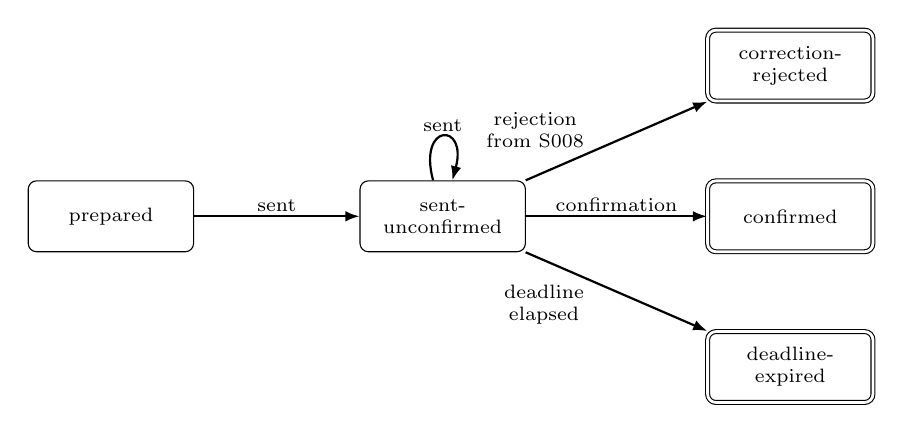
\begin{tikzpicture}[
  node distance=1.0cm and 1.5cm,
  st/.style={draw, rounded corners=3pt, align=center, font=\scriptsize,
             minimum width=2.1cm, minimum height=0.9cm},
  konac/.style={st, double, double distance=1pt},
  pr/.style={-{Latex[length=1.8mm]}, thick},
  ozn/.style={font=\scriptsize, align=center, inner sep=1.5pt}
]
  \node[st] (pri) {prepared};
  \node[st, right=2.1cm of pri] (nep) {sent-\\unconfirmed};
  \node[konac, right=2.3cm of nep] (pot) {confirmed};
  \node[konac, above=1.0cm of pot] (odb) {correction-\\rejected};
  \node[konac, below=1.0cm of pot] (rok) {deadline-\\expired};

  \draw[pr] (pri) -- node[ozn, above] {sent} (nep);
  \draw[pr] (nep) -- node[ozn, above] {confirmation} (pot);
  \draw[pr] (nep) -- node[ozn, above left, pos=0.35] {rejection\\from S008} (odb);
  \draw[pr] (nep) -- node[ozn, below left, pos=0.35] {deadline\\elapsed} (rok);
  \draw[pr] (nep) to[loop above] node[ozn, above] {sent} (nep);
\end{tikzpicture}
\caption[Automat predaje dokumenta]{Automat predaje. Dvostruki obrub označava
stanje iz kojeg nema prijelaza. Izostanak odgovora nije prijelaz nego petlja:
dokument koji je poslan i nije potvrđen ostaje poslan i nepotvrđen.}
\label{fig:automat}
\end{figure}

Rok iz članka 49.\ stavka 1.\ u automat ne ulazi kao stanje nego kao uvjet nad
prijelazom, iz razloga koji daje odjeljak~\ref{sec:automat}.
Listing~\ref{lst:automat} pokazuje taj uvjet.

\begin{lstlisting}[language=PHP, caption={[Tablica prijelaza i uvjet
roka]Tablica prijelaza i uvjet roka. Prijelaz pokreće poticaj, a rok samo
odlučuje je li poticaj dopušten.}, label={lst:automat}]
private const TRANSITIONS = [
    State::PREPARED->value => [
        Trigger::SENT->value => State::SENT_UNCONFIRMED,
    ],
    State::SENT_UNCONFIRMED->value => [
        Trigger::SENT->value                   => State::SENT_UNCONFIRMED,
        Trigger::CONFIRMATION->value           => State::CONFIRMED,
        Trigger::CONFIRMATION_FROM_S008->value => State::CONFIRMED,
        Trigger::REJECTION_FROM_S008->value    => State::CORRECTION_REJECTED,
        Trigger::DEADLINE_ELAPSED->value       => State::DEADLINE_EXPIRED,
    ],
];

// Rok kao uvjet nad prijelazom, ne kao stanje.
if ($trigger === Trigger::SENT && $expired) {
    throw new DomainException(
        'Ponovno slanje nije dopusteno: rok iz cl. 49. st. 1. je istrosen.'
    );
}
\end{lstlisting}

Nedopušten prijelaz baca iznimku i ne mijenja stanje. Sustav koji nedopušten
prijelaz tiho preskoči prestaje biti dokaz o vlastitom stanju.

Predaja se u odlazni pretinac zapisuje prije poziva, u istoj transakciji u
kojoj nastaje dokument, uz ključ koji određuje
pošiljatelj\cite{saltzer1984endtoend}. Zapisana namjera nosi i drugi posao,
teži od prvog. Listing~\ref{lst:s008} pokazuje mjesto na kojem se šifra S008
tumači.

\begin{lstlisting}[language=PHP, caption={[Tumačenje šifre S008 uz zapisanu
namjeru]Tumačenje šifre S008. Ista šifra vodi u dva suprotna prijelaza, a
razlučuje ih samo namjera zapisana prije slanja.}, label={lst:s008}]
return match ($intent) {
    Intent::RETRY => Interpretation::unambiguous(
        Trigger::CONFIRMATION_FROM_S008,
        'S008 uz zapisan ponovni pokusaj dokazuje da je raniji pokusaj prosao',
    ),

    Intent::CORRECTION => Interpretation::unambiguous(
        Trigger::REJECTION_FROM_S008,
        'S008 uz zapisan ispravak znaci odbijenicu propisanog tijeka ispravka',
    ),

    null => Interpretation::ambiguous(
        'S008 bez zapisane namjere: ista sifra znaci i potvrdu i odbijenicu',
    ),
};
\end{lstlisting}

Zadnji slučaj u listingu je onaj koji se ne smije prešutjeti. Kada zapisa
nema, funkcija ne pogađa nego vraća dvoznačan ishod, a automat tada nema
prijelaz na raspolaganju. Rupa ostaje vidljiva umjesto da se popuni
pretpostavkom.

U evidenciju ulazi svaki prijelaz, ali i svaki trenutak u kojem tumačenje nije
bilo jednoznačno. To drugo je ono zbog čega tablica postoji.

% ------------------------------------------------------------
\section{Scenariji i ishodi}
\label{sec:scenariji}
% ⚠ SVI ISPISI SU STVARNI, uzeti 2026-08-13. Sat prototipa je fiksiran
%   na 2026-09-01 09:00:00, pa su ponovljivi. Ako se kod mijenja,
%   ISPISE UZETI PONOVO.
%
% ★ SVAKI scenarij završava rečenicom koja imenuje ĆELIJU matrice.

Tri scenarija pokrivaju po jedan način otkazivanja iz
odjeljka~\ref{sec:failure-modes}. Svaki se pokreće u obje izvedbe, sa zapisom
namjere i bez njega. Sat je pritom zamrznut na jedan trenutak, pa su ispisi
ponovljivi.

\begin{table}[htbp]
\centering
\caption[Scenariji i završna stanja]{Scenariji i završna stanja. Razlika među
stupcima nastaje samo iz trenutka u kojem se zapisuje namjera.}
\label{tab:scenariji}
\small
\begin{tabular}{@{}llll@{}}
\toprule
& Odgovor & Sa zapisom namjere & Bez zapisa namjere \\
\midrule
B1 & izostaje       & \texttt{sent-unconfirmed}    & nema zapisa \\
E1 & izostaje       & predaja bez potvrde: 1       & predaja bez potvrde: 0 \\
B2 & S008 uz ispravak & \texttt{correction-rejected} & \texttt{sent-unconfirmed} \\
\bottomrule
\end{tabular}
\end{table}

\paragraph{B1: poziv istekne bez odgovora.}
Sa zapisom namjere dokument završava u stanju \texttt{sent-unconfirmed}, uz
zabilježen dan nastupa nemogućnosti i zakazan sljedeći pokušaj. Bez zapisa u
bazi ne postoji nijedan redak o predaji, iako je račun izdan.

Scenarij pokazuje i zašto raspored ponavljanja mora gledati rok.
Tablica~\ref{tab:raspored} stavlja dva rasporeda jedan pokraj drugog.

\begin{table}[htbp]
\centering
\caption[Raspored ponavljanja prema roku i prema broju pokušaja]{Raspored
ponavljanja uz rok koji istječe 8.~rujna u 23:59:59. Lijevi stupac gleda
preostali rok, desni samo broj dotadašnjih pokušaja.}
\label{tab:raspored}
\small
\begin{tabular}{@{}ccc@{}}
\toprule
Pokušaj & Svjestan roka & Eksponencijalni odmak \\
\midrule
1 & 2026-09-05 04:29:59 & 2026-09-01 09:01:00 \\
2 & 2026-09-07 02:14:59 & 2026-09-01 09:03:00 \\
3 & 2026-09-08 01:07:29 & 2026-09-01 09:07:00 \\
4 & 2026-09-08 12:33:44 & 2026-09-01 09:15:00 \\
5 & 2026-09-08 18:16:51 & 2026-09-01 09:31:00 \\
\bottomrule
\end{tabular}
\end{table}

Nalaz je precizniji od očekivanog. Eksponencijalni odmak rok ne probija rano
nego ga uopće ne dodiruje. Prvih pet pokušaja potroši u trideset i jednoj
minuti, a rok prekorači tek na četrnaestom. Mana obrasca ovdje nije da kasni.
Mana je da mu raspored s rokom nema nikakve veze, pa se isti obrazac uz
drukčiju osnovicu ponaša posve drukčije, a propis se u tom izboru ne
pojavljuje. Raspored svjestan roka svaki pokušaj stavlja na polovicu
preostalog roka i zato ga po konstrukciji ne može prekoračiti. Brookerovo
slučajno raspršivanje razmaka isključeno je, da ispis ostane
ponovljiv\cite{brookertimeouts}.

Scenarij popunjava ćelije B1 uz automat s imenovanim stanjem i B1 uz
ponavljanje svjesno roka.

\paragraph{E1: predaja bez potvrde.}
Pitanje na koje scenarij odgovara nije je li dokument stigao. Pitanje je može
li poslovni sustav znati da ga je pokušao predati. Sa zapisom namjere odgovor
postoji i provjerljiv je bez pristupa pristupnoj točki. Bez zapisa račun
postoji, a trag predaje ne postoji.

Scenarij popunjava ćeliju E1 uz odlazni pretinac i zapis namjere.

\paragraph{B2: ista šifra za dva ishoda.}
Scenarij ima dva dijela. U prvom se poruka ponavlja nakon isteka vremena i
dobiva S008. U drugom se šalje ispravak pod istim brojem računa i dobiva istu
šifru. Listing~\ref{lst:ispis} prepisuje završno stanje baze.

\begin{lstlisting}[caption={[Završno stanje baze nakon scenarija
B2]Završno stanje nakon scenarija B2, izlaz naredbe \texttt{php artisan
state}. Ista šifra, dva različita završna stanja.}, label={lst:ispis}]
PREDAJE
+----+------------+------------+---------------------+------+---------+
| id | racun      | namjera    | stanje              | pok. | odgovor |
+----+------------+------------+---------------------+------+---------+
| 1  | R-2026-003 | retry      | confirmed           | 2    | s008    |
| 2  | R-2026-003 | correction | correction-rejected | 1    | s008    |
+----+------------+------------+---------------------+------+---------+

EVIDENCIJA
+---------+-----+------------------------+------------------+-------------+
| predaja | br. | dogadaj                | u                | jednoznacno |
+---------+-----+------------------------+------------------+-------------+
| 1       | 1   | zapisana namjera       | prepared         | da          |
| 1       | 2   | sent                   | sent-unconfirmed | da          |
| 1       | 3   | tumacenje odgovora     | sent-unconfirmed | NE          |
| 1       | 4   | sent                   | sent-unconfirmed | da          |
| 1       | 5   | confirmation-from-s008 | confirmed        | da          |
+---------+-----+------------------------+------------------+-------------+
\end{lstlisting}

Treći redak evidencije je onaj koji nosi tezu poglavlja. Sustav je u tom
trenutku znao da ne zna, i to je zapisao. Kasniji odgovor S008 taj trenutak
razrješava, ali ga ne briše.

Bez zapisa namjere oba dijela scenarija završavaju u istom stanju,
\texttt{sent-unconfirmed}. Dvije suprotne namjere, ista šifra i isti ishod.
To je slučaj B2 u izvedbi.

Scenarij popunjava ćeliju B2 uz odlazni pretinac i zapis namjere.

% ------------------------------------------------------------
% TVRDNJE KAO TESTOVI — veza s metodom iz pogl. 8.
% CoFI [chen2020cofi] i Filibuster [meiklejohn2021filibuster] su citirani
% u 8.1 kao opravdanje metode; ovdje se citira samo OBLIK tvrdnje.

Svaka tvrdnja iz ovog odjeljka zapisana je i kao izvršni test, u obliku koji
Filibuster koristi za uvjetne tvrdnje\cite{meiklejohn2021filibuster}. Test ne
provjerava da je poziv uspio nego da je završno stanje ono koje propis i
obrazac zajedno nalažu. Prototip nosi dvadeset i tri takve tvrdnje, a
poglavlje~\ref{ch:evaluacija} poziva se na njih kada ćeliju označava kao
pokazanu.


% ============================================================
%  8. Evaluacija
%  Odjeljke definira: magla — graduira nakon mjerenja
% ============================================================
\chapter{Evaluacija}
\label{ch:evaluacija}

\todo{Scenariji kvarova, presuda oraclea, rezultati po stepenicama ljestvice. Tablice se GENERIRAJU iz harnessa, ne prepisuju rukom.}

% ============================================================
%  9. Rasprava
%  Odjeljke definira: magla — graduira nakon evaluacije
% ============================================================
\chapter{Rasprava}
\label{ch:rasprava}

\todo{Marginalni doprinos i cijena po uzorku; što ostaje nesvodivo; kompromisi i praktične implikacije; ograničenja evaluacije.}

% ============================================================
%  10. Zakljucak
%  Odjeljke definira: magla — pise se zadnji
% ============================================================
\chapter{Zaključak}
\label{ch:zakljucak}

\todo{Sažetak doprinosa, odgovori na RQ1-RQ3, buduće nadogradnje.}


% ---- Prilozi -----------------------------------------------
% Numeracija poglavlja prelazi u slova (Prilog A, B, ...).
\appendix
% ============================================================
%  Prilog: preostale šutnje propisa
%  Jedanaest slučajeva razrađeno je u 6.2, a preostalih sedam ide u
%  prilog kao tablica s citatima.
%
%  S12 je provjeren 2026-08-14: Pravilnik o eRačunu (NN 11/2026, 21 članak)
%    ne sadrži
%    nijednu pojavu riječi "nedostupnost". Dvoznačnost čl. 40. dakle
%    ostaje. Oznaka zatvorena.
%
%  ⚠ S23 je provjeren doslovno na izvoru 2026-08-14 i stranica je
%    arhivirana u rad/izvori/ uz SHA-256, jer nema pročišćen tekst.
% ============================================================
\chapter{Preostale šutnje propisa}
\label{ch:prilog-sutnje}

Odjeljak~\ref{sec:failure-modes} razradio je jedanaest načina otkazivanja koji
imaju posljedicu na zakonsku obvezu. Tijekom izvoda utvrđeno je još sedam mjesta
na kojima propis ne kaže ono što bi izvedba trebala znati. Ona nemaju vlastiti
način otkazivanja, ili ga imaju posredno, pa su ostavljena ovdje uz citate.

Tablica~\ref{tab:sutnje} nije popis primjedbi. Svaka stavka je mjesto na kojem
izvedba mora odlučiti nešto što propis nije odlučio, a takva odluka se ne može
obraniti pozivom na izvor.

\begin{table}[htbp]
\centering
\caption[Preostale šutnje propisa]{Mjesta na kojima propis ne daje podatak koji
izvedba treba. Oznake slijede numeraciju iz izvoda.}
\label{tab:sutnje}
\scriptsize
\setlength{\tabcolsep}{4pt}
\renewcommand{\arraystretch}{1.25}
\begin{tabular}{@{}p{0.7cm}p{5.4cm}p{8.4cm}@{}}
\toprule
& \textsc{Šutnja} & \textsc{Što izvedba mora odlučiti sama} \\
\midrule

S12 & Nedostupnost AMS-a kao servisa nije uređena &
Članak 40.\ pokriva nedostupnost \emph{identifikatora} u AMS-u, dakle slučaj u
kojem se primatelj nije registrirao. Ispad samog servisa gramatički nije
pokriven. Pravilnik tu dvoznačnost ne razrješava. \\

S13 & Nema izlaza za rad bez veze &
Za promet u krajnjoj potrošnji postoje uvezana knjiga računa (čl.~22.) i potvrda
regulatora (čl.~23.). U dijelu o eRačunu ekvivalenta nema. Jedini papirnati
izlaz vezan je isključivo na AMS (čl.~40.~st.~2.). \\

S14 & „Zadovoljavajuća podrška“ nije kvantificirana &
Članak 49.\ stavak 2.\ traži zadovoljavajuću programsku i sklopovsku podršku, a
mjeru ne daje. Izostanak podrške je teži prekršaj
(čl.~72.~st.~1.~t.~10.), pa se sankcionira uvjet koji nije mjerljiv. \\

S19 & Referencijalni integritet reference na prethodni račun &
Nijedno pravilo ne traži da referencirani prethodni račun postoji, da je poslan
ni da je zaprimljen. Schematron traži samo da polje ne bude prazno kada je
skupina prisutna\cite{cen2026validationartefacts}. \\

S20 & Storno nema opisan životni ciklus &
Norma ne poznaje tip dokumenta za poništenje\cite{cen2019en16931}. Hrvatsko
suženje dodaje procesni kod, ali ne određuje semantiku
obrade\cite{pu2026hrcius}. Članak 52.\ stavak 4.\ storniranje ostavlja
mogućnošću, a rok u kojem primatelj smije odbiti nije propisan. \\

S21 & Čuvanje i ponovno izvođenje fiskalizacijskih poruka &
Članak 35.\ propisuje čuvanje eRačuna u izvornom obliku šest godina. O čuvanju
fiskalizacijskih poruka, odgovora i zapisa ne kaže ništa, kao ni o pravu ili
obvezi ponovnog izvođenja tijeka. Europski profil rok čuvanja dokaza
neporecivosti prepušta politici koju nijedan dokument ne
donosi\cite{cef2020as4v115}. \\

S23 & Semantika duplikata živi izvan propisa &
Pravilo da se eRačun pod istim brojem smije poslati samo jednom, obveza
pristupne točke primatelja da vrati potvrdu neovisno o tome je li dokument već
zaprimila i postupanje s tehničkim duplikatom razrađeni su isključivo u rubrici
pitanja i odgovora\cite{pu2026pitanjaodgovori}. Ni Zakon, ni Pravilnik, ni
tehnička specifikacija taj obrazac ne sadrže. \\

\bottomrule
\end{tabular}
\end{table}

Posljednja stavka ima drukčiju narav od ostalih šest i zato je razrađena u
odjeljku~\ref{sec:ogranicenja}. Kod nje propis ne šuti zato što pitanje nije
uočeno. Odgovor postoji i mjerodavan je, ali stoji u dokumentu koji nije propis
i koji se mijenja bez pročišćenog teksta.


% ---- Literatura --------------------------------------------
\backmatter
\printbibliography[heading=bibintoc,title={Literatura}]

% ---- Popis nedovršenog -------------------------------------
% Uklonjen 2026-08-14, jer nijedna \todo oznaka više ne postoji.
% Naredbe \todo i \popistodo ostaju u preambuli. Ako se u doradi
% pojavi nova oznaka, vratiti \popistodo ovamo da se ne izgubi
% iz vida, i ukloniti ga opet prije predaje.
% \popistodo

\end{document}
